%% fig_vgscope.tex   (generated by make_round41.py; do not edit by hand)
%% The Hodge conjecture for the very general complete intersection X_{d,r}(lambda), every N (thm:vgvandermonde, rem:vandermonde).
\documentclass[tikz,border=8pt]{standalone}
\usepackage{amsmath,amssymb}
\usetikzlibrary{arrows.meta,calc,decorations.pathreplacing}
%% palette.tex -- shared colour definitions for the figures
\definecolor{PInk}{RGB}{26,32,44}
\definecolor{PBlue}{RGB}{37,82,139}
\definecolor{PTeal}{RGB}{23,127,125}
\definecolor{POchre}{RGB}{193,138,44}
\definecolor{PClay}{RGB}{178,74,58}
\definecolor{PSlate}{RGB}{108,122,137}
\definecolor{PViolet}{RGB}{110,86,150}
\definecolor{WBlue}{RGB}{223,234,246}
\definecolor{WTeal}{RGB}{220,238,236}
\definecolor{WOchre}{RGB}{250,240,218}
\definecolor{WClay}{RGB}{247,229,224}
\definecolor{WSlate}{RGB}{238,241,244}
\definecolor{PMag}{RGB}{158,58,110}
\definecolor{PGrass}{RGB}{62,124,66}
\definecolor{PAmber}{RGB}{214,112,38}
\definecolor{PIndigo}{RGB}{58,64,140}
\definecolor{PRule}{RGB}{176,186,197}

%% shared macros so the standalone figures match the paper
\providecommand{\QQ}{\mathbb{Q}}
\providecommand{\ZZ}{\mathbb{Z}}
\providecommand{\RR}{\mathbb{R}}
\providecommand{\CC}{\mathbb{C}}
\providecommand{\PP}{\mathbb{P}}
\providecommand{\Kx}{K^{\times}}
\providecommand{\HW}{W}
\providecommand{\Nm}{\mathrm{N}}
\providecommand{\Hdg}{\mathrm{Hdg}}
\providecommand{\NS}{\mathrm{NS}}
\providecommand{\cA}{\mathcal{A}}
\providecommand{\cD}{\mathcal{D}}
\providecommand{\cF}{\mathcal{F}}
\providecommand{\cP}{\mathcal{P}}
\providecommand{\cO}{\mathcal{O}}
\providecommand{\cQ}{\mathcal{Q}}
\providecommand{\bbar}[1]{\overline{#1}}
\providecommand{\ch}{\operatorname{ch}}
\providecommand{\End}{\mathrm{End}}
\providecommand{\Ext}{\operatorname{Ext}}
\providecommand{\Supp}{\operatorname{Supp}}

\begin{document}
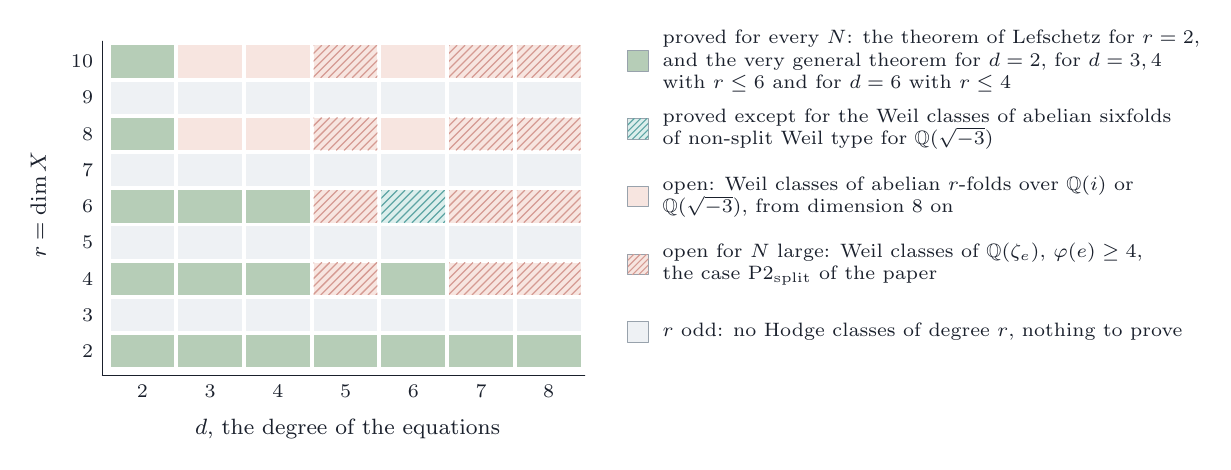
\begin{tikzpicture}[x=1cm,y=1cm,line join=round,line cap=round,
  font=\small,text=PInk,lbl/.style={inner sep=1pt}]
  \path[fill=PGrass!38!white,draw=none] (1.1000,0.0000) rectangle (1.9100,0.4100);
  \path[fill=WSlate,draw=none] (1.1000,0.4600) rectangle (1.9100,0.8700);
  \path[fill=PGrass!38!white,draw=none] (1.1000,0.9200) rectangle (1.9100,1.3300);
  \path[fill=WSlate,draw=none] (1.1000,1.3800) rectangle (1.9100,1.7900);
  \path[fill=PGrass!38!white,draw=none] (1.1000,1.8400) rectangle (1.9100,2.2500);
  \path[fill=WSlate,draw=none] (1.1000,2.3000) rectangle (1.9100,2.7100);
  \path[fill=PGrass!38!white,draw=none] (1.1000,2.7600) rectangle (1.9100,3.1700);
  \path[fill=WSlate,draw=none] (1.1000,3.2200) rectangle (1.9100,3.6300);
  \path[fill=PGrass!38!white,draw=none] (1.1000,3.6800) rectangle (1.9100,4.0900);
  \path[fill=PGrass!38!white,draw=none] (1.9600,0.0000) rectangle (2.7700,0.4100);
  \path[fill=WSlate,draw=none] (1.9600,0.4600) rectangle (2.7700,0.8700);
  \path[fill=PGrass!38!white,draw=none] (1.9600,0.9200) rectangle (2.7700,1.3300);
  \path[fill=WSlate,draw=none] (1.9600,1.3800) rectangle (2.7700,1.7900);
  \path[fill=PGrass!38!white,draw=none] (1.9600,1.8400) rectangle (2.7700,2.2500);
  \path[fill=WSlate,draw=none] (1.9600,2.3000) rectangle (2.7700,2.7100);
  \path[fill=WClay,draw=none] (1.9600,2.7600) rectangle (2.7700,3.1700);
  \path[fill=WSlate,draw=none] (1.9600,3.2200) rectangle (2.7700,3.6300);
  \path[fill=WClay,draw=none] (1.9600,3.6800) rectangle (2.7700,4.0900);
  \path[fill=PGrass!38!white,draw=none] (2.8200,0.0000) rectangle (3.6300,0.4100);
  \path[fill=WSlate,draw=none] (2.8200,0.4600) rectangle (3.6300,0.8700);
  \path[fill=PGrass!38!white,draw=none] (2.8200,0.9200) rectangle (3.6300,1.3300);
  \path[fill=WSlate,draw=none] (2.8200,1.3800) rectangle (3.6300,1.7900);
  \path[fill=PGrass!38!white,draw=none] (2.8200,1.8400) rectangle (3.6300,2.2500);
  \path[fill=WSlate,draw=none] (2.8200,2.3000) rectangle (3.6300,2.7100);
  \path[fill=WClay,draw=none] (2.8200,2.7600) rectangle (3.6300,3.1700);
  \path[fill=WSlate,draw=none] (2.8200,3.2200) rectangle (3.6300,3.6300);
  \path[fill=WClay,draw=none] (2.8200,3.6800) rectangle (3.6300,4.0900);
  \path[fill=PGrass!38!white,draw=none] (3.6800,0.0000) rectangle (4.4900,0.4100);
  \path[fill=WSlate,draw=none] (3.6800,0.4600) rectangle (4.4900,0.8700);
  \path[fill=WClay,draw=none] (3.6800,0.9200) rectangle (4.4900,1.3300);
  \begin{scope}\clip (3.6800,0.9200) rectangle (4.4900,1.3300);\draw[PClay!55,line width=0.45pt] (3.2700,0.9200) -- (3.6800,1.3300) (3.3700,0.9200) -- (3.7800,1.3300) (3.4700,0.9200) -- (3.8800,1.3300) (3.5700,0.9200) -- (3.9800,1.3300) (3.6700,0.9200) -- (4.0800,1.3300) (3.7700,0.9200) -- (4.1800,1.3300) (3.8700,0.9200) -- (4.2800,1.3300) (3.9700,0.9200) -- (4.3800,1.3300) (4.0700,0.9200) -- (4.4800,1.3300) (4.1700,0.9200) -- (4.5800,1.3300) (4.2700,0.9200) -- (4.6800,1.3300) (4.3700,0.9200) -- (4.7800,1.3300) (4.4700,0.9200) -- (4.8800,1.3300);\end{scope}
  \path[fill=WSlate,draw=none] (3.6800,1.3800) rectangle (4.4900,1.7900);
  \path[fill=WClay,draw=none] (3.6800,1.8400) rectangle (4.4900,2.2500);
  \begin{scope}\clip (3.6800,1.8400) rectangle (4.4900,2.2500);\draw[PClay!55,line width=0.45pt] (3.2700,1.8400) -- (3.6800,2.2500) (3.3700,1.8400) -- (3.7800,2.2500) (3.4700,1.8400) -- (3.8800,2.2500) (3.5700,1.8400) -- (3.9800,2.2500) (3.6700,1.8400) -- (4.0800,2.2500) (3.7700,1.8400) -- (4.1800,2.2500) (3.8700,1.8400) -- (4.2800,2.2500) (3.9700,1.8400) -- (4.3800,2.2500) (4.0700,1.8400) -- (4.4800,2.2500) (4.1700,1.8400) -- (4.5800,2.2500) (4.2700,1.8400) -- (4.6800,2.2500) (4.3700,1.8400) -- (4.7800,2.2500) (4.4700,1.8400) -- (4.8800,2.2500);\end{scope}
  \path[fill=WSlate,draw=none] (3.6800,2.3000) rectangle (4.4900,2.7100);
  \path[fill=WClay,draw=none] (3.6800,2.7600) rectangle (4.4900,3.1700);
  \begin{scope}\clip (3.6800,2.7600) rectangle (4.4900,3.1700);\draw[PClay!55,line width=0.45pt] (3.2700,2.7600) -- (3.6800,3.1700) (3.3700,2.7600) -- (3.7800,3.1700) (3.4700,2.7600) -- (3.8800,3.1700) (3.5700,2.7600) -- (3.9800,3.1700) (3.6700,2.7600) -- (4.0800,3.1700) (3.7700,2.7600) -- (4.1800,3.1700) (3.8700,2.7600) -- (4.2800,3.1700) (3.9700,2.7600) -- (4.3800,3.1700) (4.0700,2.7600) -- (4.4800,3.1700) (4.1700,2.7600) -- (4.5800,3.1700) (4.2700,2.7600) -- (4.6800,3.1700) (4.3700,2.7600) -- (4.7800,3.1700) (4.4700,2.7600) -- (4.8800,3.1700);\end{scope}
  \path[fill=WSlate,draw=none] (3.6800,3.2200) rectangle (4.4900,3.6300);
  \path[fill=WClay,draw=none] (3.6800,3.6800) rectangle (4.4900,4.0900);
  \begin{scope}\clip (3.6800,3.6800) rectangle (4.4900,4.0900);\draw[PClay!55,line width=0.45pt] (3.2700,3.6800) -- (3.6800,4.0900) (3.3700,3.6800) -- (3.7800,4.0900) (3.4700,3.6800) -- (3.8800,4.0900) (3.5700,3.6800) -- (3.9800,4.0900) (3.6700,3.6800) -- (4.0800,4.0900) (3.7700,3.6800) -- (4.1800,4.0900) (3.8700,3.6800) -- (4.2800,4.0900) (3.9700,3.6800) -- (4.3800,4.0900) (4.0700,3.6800) -- (4.4800,4.0900) (4.1700,3.6800) -- (4.5800,4.0900) (4.2700,3.6800) -- (4.6800,4.0900) (4.3700,3.6800) -- (4.7800,4.0900) (4.4700,3.6800) -- (4.8800,4.0900);\end{scope}
  \path[fill=PGrass!38!white,draw=none] (4.5400,0.0000) rectangle (5.3500,0.4100);
  \path[fill=WSlate,draw=none] (4.5400,0.4600) rectangle (5.3500,0.8700);
  \path[fill=PGrass!38!white,draw=none] (4.5400,0.9200) rectangle (5.3500,1.3300);
  \path[fill=WSlate,draw=none] (4.5400,1.3800) rectangle (5.3500,1.7900);
  \path[fill=WTeal,draw=none] (4.5400,1.8400) rectangle (5.3500,2.2500);
  \begin{scope}\clip (4.5400,1.8400) rectangle (5.3500,2.2500);\draw[PTeal!70,line width=0.45pt] (4.1300,1.8400) -- (4.5400,2.2500) (4.2300,1.8400) -- (4.6400,2.2500) (4.3300,1.8400) -- (4.7400,2.2500) (4.4300,1.8400) -- (4.8400,2.2500) (4.5300,1.8400) -- (4.9400,2.2500) (4.6300,1.8400) -- (5.0400,2.2500) (4.7300,1.8400) -- (5.1400,2.2500) (4.8300,1.8400) -- (5.2400,2.2500) (4.9300,1.8400) -- (5.3400,2.2500) (5.0300,1.8400) -- (5.4400,2.2500) (5.1300,1.8400) -- (5.5400,2.2500) (5.2300,1.8400) -- (5.6400,2.2500) (5.3300,1.8400) -- (5.7400,2.2500);\end{scope}
  \path[fill=WSlate,draw=none] (4.5400,2.3000) rectangle (5.3500,2.7100);
  \path[fill=WClay,draw=none] (4.5400,2.7600) rectangle (5.3500,3.1700);
  \path[fill=WSlate,draw=none] (4.5400,3.2200) rectangle (5.3500,3.6300);
  \path[fill=WClay,draw=none] (4.5400,3.6800) rectangle (5.3500,4.0900);
  \path[fill=PGrass!38!white,draw=none] (5.4000,0.0000) rectangle (6.2100,0.4100);
  \path[fill=WSlate,draw=none] (5.4000,0.4600) rectangle (6.2100,0.8700);
  \path[fill=WClay,draw=none] (5.4000,0.9200) rectangle (6.2100,1.3300);
  \begin{scope}\clip (5.4000,0.9200) rectangle (6.2100,1.3300);\draw[PClay!55,line width=0.45pt] (4.9900,0.9200) -- (5.4000,1.3300) (5.0900,0.9200) -- (5.5000,1.3300) (5.1900,0.9200) -- (5.6000,1.3300) (5.2900,0.9200) -- (5.7000,1.3300) (5.3900,0.9200) -- (5.8000,1.3300) (5.4900,0.9200) -- (5.9000,1.3300) (5.5900,0.9200) -- (6.0000,1.3300) (5.6900,0.9200) -- (6.1000,1.3300) (5.7900,0.9200) -- (6.2000,1.3300) (5.8900,0.9200) -- (6.3000,1.3300) (5.9900,0.9200) -- (6.4000,1.3300) (6.0900,0.9200) -- (6.5000,1.3300) (6.1900,0.9200) -- (6.6000,1.3300);\end{scope}
  \path[fill=WSlate,draw=none] (5.4000,1.3800) rectangle (6.2100,1.7900);
  \path[fill=WClay,draw=none] (5.4000,1.8400) rectangle (6.2100,2.2500);
  \begin{scope}\clip (5.4000,1.8400) rectangle (6.2100,2.2500);\draw[PClay!55,line width=0.45pt] (4.9900,1.8400) -- (5.4000,2.2500) (5.0900,1.8400) -- (5.5000,2.2500) (5.1900,1.8400) -- (5.6000,2.2500) (5.2900,1.8400) -- (5.7000,2.2500) (5.3900,1.8400) -- (5.8000,2.2500) (5.4900,1.8400) -- (5.9000,2.2500) (5.5900,1.8400) -- (6.0000,2.2500) (5.6900,1.8400) -- (6.1000,2.2500) (5.7900,1.8400) -- (6.2000,2.2500) (5.8900,1.8400) -- (6.3000,2.2500) (5.9900,1.8400) -- (6.4000,2.2500) (6.0900,1.8400) -- (6.5000,2.2500) (6.1900,1.8400) -- (6.6000,2.2500);\end{scope}
  \path[fill=WSlate,draw=none] (5.4000,2.3000) rectangle (6.2100,2.7100);
  \path[fill=WClay,draw=none] (5.4000,2.7600) rectangle (6.2100,3.1700);
  \begin{scope}\clip (5.4000,2.7600) rectangle (6.2100,3.1700);\draw[PClay!55,line width=0.45pt] (4.9900,2.7600) -- (5.4000,3.1700) (5.0900,2.7600) -- (5.5000,3.1700) (5.1900,2.7600) -- (5.6000,3.1700) (5.2900,2.7600) -- (5.7000,3.1700) (5.3900,2.7600) -- (5.8000,3.1700) (5.4900,2.7600) -- (5.9000,3.1700) (5.5900,2.7600) -- (6.0000,3.1700) (5.6900,2.7600) -- (6.1000,3.1700) (5.7900,2.7600) -- (6.2000,3.1700) (5.8900,2.7600) -- (6.3000,3.1700) (5.9900,2.7600) -- (6.4000,3.1700) (6.0900,2.7600) -- (6.5000,3.1700) (6.1900,2.7600) -- (6.6000,3.1700);\end{scope}
  \path[fill=WSlate,draw=none] (5.4000,3.2200) rectangle (6.2100,3.6300);
  \path[fill=WClay,draw=none] (5.4000,3.6800) rectangle (6.2100,4.0900);
  \begin{scope}\clip (5.4000,3.6800) rectangle (6.2100,4.0900);\draw[PClay!55,line width=0.45pt] (4.9900,3.6800) -- (5.4000,4.0900) (5.0900,3.6800) -- (5.5000,4.0900) (5.1900,3.6800) -- (5.6000,4.0900) (5.2900,3.6800) -- (5.7000,4.0900) (5.3900,3.6800) -- (5.8000,4.0900) (5.4900,3.6800) -- (5.9000,4.0900) (5.5900,3.6800) -- (6.0000,4.0900) (5.6900,3.6800) -- (6.1000,4.0900) (5.7900,3.6800) -- (6.2000,4.0900) (5.8900,3.6800) -- (6.3000,4.0900) (5.9900,3.6800) -- (6.4000,4.0900) (6.0900,3.6800) -- (6.5000,4.0900) (6.1900,3.6800) -- (6.6000,4.0900);\end{scope}
  \path[fill=PGrass!38!white,draw=none] (6.2600,0.0000) rectangle (7.0700,0.4100);
  \path[fill=WSlate,draw=none] (6.2600,0.4600) rectangle (7.0700,0.8700);
  \path[fill=WClay,draw=none] (6.2600,0.9200) rectangle (7.0700,1.3300);
  \begin{scope}\clip (6.2600,0.9200) rectangle (7.0700,1.3300);\draw[PClay!55,line width=0.45pt] (5.8500,0.9200) -- (6.2600,1.3300) (5.9500,0.9200) -- (6.3600,1.3300) (6.0500,0.9200) -- (6.4600,1.3300) (6.1500,0.9200) -- (6.5600,1.3300) (6.2500,0.9200) -- (6.6600,1.3300) (6.3500,0.9200) -- (6.7600,1.3300) (6.4500,0.9200) -- (6.8600,1.3300) (6.5500,0.9200) -- (6.9600,1.3300) (6.6500,0.9200) -- (7.0600,1.3300) (6.7500,0.9200) -- (7.1600,1.3300) (6.8500,0.9200) -- (7.2600,1.3300) (6.9500,0.9200) -- (7.3600,1.3300) (7.0500,0.9200) -- (7.4600,1.3300);\end{scope}
  \path[fill=WSlate,draw=none] (6.2600,1.3800) rectangle (7.0700,1.7900);
  \path[fill=WClay,draw=none] (6.2600,1.8400) rectangle (7.0700,2.2500);
  \begin{scope}\clip (6.2600,1.8400) rectangle (7.0700,2.2500);\draw[PClay!55,line width=0.45pt] (5.8500,1.8400) -- (6.2600,2.2500) (5.9500,1.8400) -- (6.3600,2.2500) (6.0500,1.8400) -- (6.4600,2.2500) (6.1500,1.8400) -- (6.5600,2.2500) (6.2500,1.8400) -- (6.6600,2.2500) (6.3500,1.8400) -- (6.7600,2.2500) (6.4500,1.8400) -- (6.8600,2.2500) (6.5500,1.8400) -- (6.9600,2.2500) (6.6500,1.8400) -- (7.0600,2.2500) (6.7500,1.8400) -- (7.1600,2.2500) (6.8500,1.8400) -- (7.2600,2.2500) (6.9500,1.8400) -- (7.3600,2.2500) (7.0500,1.8400) -- (7.4600,2.2500);\end{scope}
  \path[fill=WSlate,draw=none] (6.2600,2.3000) rectangle (7.0700,2.7100);
  \path[fill=WClay,draw=none] (6.2600,2.7600) rectangle (7.0700,3.1700);
  \begin{scope}\clip (6.2600,2.7600) rectangle (7.0700,3.1700);\draw[PClay!55,line width=0.45pt] (5.8500,2.7600) -- (6.2600,3.1700) (5.9500,2.7600) -- (6.3600,3.1700) (6.0500,2.7600) -- (6.4600,3.1700) (6.1500,2.7600) -- (6.5600,3.1700) (6.2500,2.7600) -- (6.6600,3.1700) (6.3500,2.7600) -- (6.7600,3.1700) (6.4500,2.7600) -- (6.8600,3.1700) (6.5500,2.7600) -- (6.9600,3.1700) (6.6500,2.7600) -- (7.0600,3.1700) (6.7500,2.7600) -- (7.1600,3.1700) (6.8500,2.7600) -- (7.2600,3.1700) (6.9500,2.7600) -- (7.3600,3.1700) (7.0500,2.7600) -- (7.4600,3.1700);\end{scope}
  \path[fill=WSlate,draw=none] (6.2600,3.2200) rectangle (7.0700,3.6300);
  \path[fill=WClay,draw=none] (6.2600,3.6800) rectangle (7.0700,4.0900);
  \begin{scope}\clip (6.2600,3.6800) rectangle (7.0700,4.0900);\draw[PClay!55,line width=0.45pt] (5.8500,3.6800) -- (6.2600,4.0900) (5.9500,3.6800) -- (6.3600,4.0900) (6.0500,3.6800) -- (6.4600,4.0900) (6.1500,3.6800) -- (6.5600,4.0900) (6.2500,3.6800) -- (6.6600,4.0900) (6.3500,3.6800) -- (6.7600,4.0900) (6.4500,3.6800) -- (6.8600,4.0900) (6.5500,3.6800) -- (6.9600,4.0900) (6.6500,3.6800) -- (7.0600,4.0900) (6.7500,3.6800) -- (7.1600,4.0900) (6.8500,3.6800) -- (7.2600,4.0900) (6.9500,3.6800) -- (7.3600,4.0900) (7.0500,3.6800) -- (7.4600,4.0900);\end{scope}
  \draw[PInk,line width=0.5pt] (1.0000,-0.1000) -- (7.1200,-0.1000);
  \draw[PInk,line width=0.5pt] (1.0000,-0.1000) -- (1.0000,4.1400);
  \path[fill=PGrass!38!white,draw=PSlate!70,line width=0.35pt] (7.6700,3.7600) rectangle (7.9300,4.0200);
  \path[fill=WTeal,draw=PSlate!70,line width=0.35pt] (7.6700,2.9000) rectangle (7.9300,3.1600);
  \begin{scope}\clip (7.6700,2.9000) rectangle (7.9300,3.1600);\draw[PTeal!70,line width=0.40pt] (7.4100,2.9000) -- (7.6700,3.1600) (7.4900,2.9000) -- (7.7500,3.1600) (7.5700,2.9000) -- (7.8300,3.1600) (7.6500,2.9000) -- (7.9100,3.1600) (7.7300,2.9000) -- (7.9900,3.1600) (7.8100,2.9000) -- (8.0700,3.1600) (7.8900,2.9000) -- (8.1500,3.1600);\end{scope}
  \path[fill=WClay,draw=PSlate!70,line width=0.35pt] (7.6700,2.0400) rectangle (7.9300,2.3000);
  \path[fill=WClay,draw=PSlate!70,line width=0.35pt] (7.6700,1.1800) rectangle (7.9300,1.4400);
  \begin{scope}\clip (7.6700,1.1800) rectangle (7.9300,1.4400);\draw[PClay!55,line width=0.40pt] (7.4100,1.1800) -- (7.6700,1.4400) (7.4900,1.1800) -- (7.7500,1.4400) (7.5700,1.1800) -- (7.8300,1.4400) (7.6500,1.1800) -- (7.9100,1.4400) (7.7300,1.1800) -- (7.9900,1.4400) (7.8100,1.1800) -- (8.0700,1.4400) (7.8900,1.1800) -- (8.1500,1.4400);\end{scope}
  \path[fill=WSlate,draw=PSlate!70,line width=0.35pt] (7.6700,0.3200) rectangle (7.9300,0.5800);
  \node[lbl,anchor=north,text=PInk,font=\scriptsize] at (1.5050,-0.1800) {$2$};
  \node[lbl,anchor=north,text=PInk,font=\scriptsize] at (2.3650,-0.1800) {$3$};
  \node[lbl,anchor=north,text=PInk,font=\scriptsize] at (3.2250,-0.1800) {$4$};
  \node[lbl,anchor=north,text=PInk,font=\scriptsize] at (4.0850,-0.1800) {$5$};
  \node[lbl,anchor=north,text=PInk,font=\scriptsize] at (4.9450,-0.1800) {$6$};
  \node[lbl,anchor=north,text=PInk,font=\scriptsize] at (5.8050,-0.1800) {$7$};
  \node[lbl,anchor=north,text=PInk,font=\scriptsize] at (6.6650,-0.1800) {$8$};
  \node[lbl,anchor=east,text=PInk,font=\scriptsize] at (0.9200,0.2050) {$2$};
  \node[lbl,anchor=east,text=PInk,font=\scriptsize] at (0.9200,0.6650) {$3$};
  \node[lbl,anchor=east,text=PInk,font=\scriptsize] at (0.9200,1.1250) {$4$};
  \node[lbl,anchor=east,text=PInk,font=\scriptsize] at (0.9200,1.5850) {$5$};
  \node[lbl,anchor=east,text=PInk,font=\scriptsize] at (0.9200,2.0450) {$6$};
  \node[lbl,anchor=east,text=PInk,font=\scriptsize] at (0.9200,2.5050) {$7$};
  \node[lbl,anchor=east,text=PInk,font=\scriptsize] at (0.9200,2.9650) {$8$};
  \node[lbl,anchor=east,text=PInk,font=\scriptsize] at (0.9200,3.4250) {$9$};
  \node[lbl,anchor=east,text=PInk,font=\scriptsize] at (0.9200,3.8850) {$10$};
  \node[lbl,anchor=north,text=PInk,font=\footnotesize] at (4.1100,-0.6200) {$d$, the degree of the equations};
  \node[lbl,anchor=south,text=PInk,font=\footnotesize,rotate=90] at (0.3200,2.0700) {$r=\dim X$};
  \node[lbl,anchor=west,text=PInk,font=\scriptsize,align=left] at (8.0700,3.8900) {proved for every $N$: the theorem of Lefschetz for $r=2$,\\ and the very general theorem for $d=2$, for $d=3,4$\\ with $r\le6$ and for $d=6$ with $r\le4$};
  \node[lbl,anchor=west,text=PInk,font=\scriptsize,align=left] at (8.0700,3.0300) {proved except for the Weil classes of abelian sixfolds\\ of non-split Weil type for $\QQ(\sqrt{-3})$};
  \node[lbl,anchor=west,text=PInk,font=\scriptsize,align=left] at (8.0700,2.1700) {open: Weil classes of abelian $r$-folds over $\QQ(i)$ or\\ $\QQ(\sqrt{-3})$, from dimension $8$ on};
  \node[lbl,anchor=west,text=PInk,font=\scriptsize,align=left] at (8.0700,1.3100) {open for $N$ large: Weil classes of $\QQ(\zeta_{e})$, $\varphi(e)\ge4$,\\ the case $\mathrm{P2}_{\mathrm{split}}$ of the paper};
  \node[lbl,anchor=west,text=PInk,font=\scriptsize,align=left] at (8.0700,0.4500) {$r$ odd: no Hodge classes of degree $r$, nothing to prove};
\end{tikzpicture}
\end{document}
